% !TEX program = pdflatex
\documentclass[10pt,a4paper]{article}
\usepackage[utf8]{inputenc}
\usepackage[T1]{fontenc}
\usepackage{geometry}
\geometry{margin=1in}
\usepackage{amsmath,amssymb,mathtools}
\usepackage{graphicx}
\usepackage{booktabs}
\usepackage{siunitx}
\sisetup{round-mode=places,round-precision=2,detect-weight=true,detect-family=true}
\usepackage{enumitem}
\usepackage{algorithm}
\usepackage{algpseudocode}
\usepackage{xcolor}
\usepackage{hyperref}
\usepackage{tikz}
\usetikzlibrary{arrows.meta,positioning,calc,fit,backgrounds,shapes.geometric,matrix}
\usepackage{cleveref}
\usepackage{paracol}
\usepackage{caption}
\hypersetup{colorlinks=true,linkcolor=blue,citecolor=blue,urlcolor=blue}

% Convenience placeholders
\newcommand{\xx}{\texttt{XXX.XX}} % mocked numeric result
\newcommand{\na}{\textemdash}      % not available

\title{Learning Sparse Feature-Interaction Graphs with Attention-Based GNNs}
\author{Phaphontee Yamchote\\ Advisor: Asst. Prof. Thanapon Noraset, Ph.D. \\ Co-advisor: Chainarong Amornbunchornvej, Ph.D.}
\date{}

\begin{document}
\maketitle

\begin{abstract}
This paper studies whether an attention-based Graph Neural Network (GNN) can capture interaction groups and select a sparse feature graph on the dataset containing interactions with known ground truth. Features are treated as nodes in a complete graph; a one-layer TransformerConv is trained to obtain attention coefficients, which are aggregated into a symmetric, min–max–normalized edge score (MF). A single global threshold $\tau$ selects edges, and the predictor is retrained on the pruned graph.

On a synthetic dataset with higher-order interactions, the method highlights the true groups: with $\tau{=}0.68$, it selects 9 edges (vs.\ 45 in the complete graph; 8 in the ground truth) and achieves Precision $0.89$, Recall $1.00$, and $F_1{=}0.94$ for edge recovery. Predictive accuracy is preserved or improved: MAE is $0.072$ for the pruned graph, compared with $0.088$ on the complete graph, $0.070$ for a ground-truth oracle, and $0.397$ for a null (no-edge) graph. These results suggest that removing noisy edges yields a compact, interpretable graph without harming prediction. The procedure is generic and can be tested on any synthetic dataset that provides ground-truth interactions for evaluation.
\end{abstract}



\section{Introduction}
Feature interaction, behavior of data whose two or more independent variables exhibit an interaction effect on their dependent variable, is one of the interesting challenges in tabular prediction\cite{molnar2020interpretable}. Models that effectively capture these interactions tend to improve accuracy. An active research area involves representing possible interactions through a \emph{feature graph}, where each feature acts as a node and edges indicate potential interactions that a graph neural network (GNN) can aggregate. Although this representation is not yet widely adopted, it provides a valuable perspective for analyzing interaction structures, especially in controlled environments. However, fully connected feature graphs result in $O(d^2)$ edges, raising noise, computational costs, and reducing interpretability. This underscores the need for a \emph{sparse} interaction graph that retains only the most informative edges.

In this paper, we study the problem in a controlled setting with known ground truth. The Table2Graph \cite{Table2Graph} synthetic dataset defines higher-order \emph{interaction groups}, allowing us to assess if a method can uncover the structure by utilizing pairwise edges as representatives for the groups. We treat structure construction as the primary goal and focus on a single dataset for a clear, controlled study.

Classical interaction models such as factorization-machine families (e.g., FM \cite{FM}, AFM \cite{AFM}, NFM\cite{He2017NeuralFM}, DeepFM \cite{DeepFM}) weight pairwise or higher-order terms, but the learned interactions are often implicit and less interpretable. Recent graph-based methods (e.g., Fi-GNN \cite{fignn}, GraphFM \cite{GraphFM}, Table2Graph \cite{Table2Graph}) operate on feature graphs and use attention or other weights to emphasize important edges. However, the specific question of \emph{how to select a sparse interaction graph}—and how well the selected edges recover ground-truth interaction groups on a controlled dataset—remains less systematically examined.

We ask whether an attention-based GNN trained on a complete feature graph can (i) expose interaction structure through its attention scores and (ii) support a simple pruning step to construct a sparser graph that keeps informative interactions. We evaluate success by edge-level Precision/Recall/F1 against the known interaction pairs and by predictive metrics on the synthetic task.

We adopt a minimal score–prune–retrain pipeline: (1) train an attention-based GNN to obtain an attention-derived edge metric; (2) prune edges by a global threshold $\tau$; and (3) retrain on the pruned graph. The pipeline targets interpretability and efficiency while keeping the modeling simple.

The principal contributions of our work are as follows:
\begin{enumerate}
    \item \textbf{Formulation:} an attention-guided \emph{feature-graph selection} setup on the synthetic dataset with known interaction groups (focusing on a single, global-threshold rule).
    \item \textbf{Evaluation protocol:} edge-level Precision/Recall/F1 for interaction-group recovery under ground truth, plus standard predictive metrics.
    \item \textbf{Evidence:} threshold-based pruning yields a sparse graph that closely matches the true interaction structure while preserving prediction quality on the synthetic task.
\end{enumerate}
We restrict the study to the single synthetic dataset to provide a clear measurement of interaction-group discovery. Pairwise edges serve as proxies for higher-order groups in this dataset; model-dependent scores may miss weak effects, which we discuss in the limitations.

\section{Related Work}\label{sec:related}
\subsection{Feature Interaction Modeling}
Feature interaction occurs when the joint effect of several features cannot be written as a sum of independent contributions. A functional ANOVA view expresses a predictor as
\begin{equation}
\small
f(\mathbf{x}) \;=\; g_0 \;+\; \sum_j g_j(x_j) \;+\; \sum_{j<k} g_{jk}(x_j,x_k) \;+\; \cdots,
\end{equation}
where non-zero interaction terms (e.g., $g_{jk}, g_{jkl}$) indicate pairwise or higher-order dependencies~\cite{herbinger2024decomposing}. Related formulations define interaction by ruling out decompositions of the form
$f(\mathbf{x})=\sum_{i\in I} g_i(x_i)+h(\mathbf{x}_{\setminus I})$ for a subset $I$, i.e., the contribution of $I$ is non-additive~\cite{tsang2020interaction,Tsang2020HowDT}.

Classical models include \emph{Factorization Machines (FM)} that capture second-order interactions via inner products of feature embeddings~\cite{FM}. Deep extensions such as \emph{Neural FM (NFM)}~\cite{He2017NeuralFM} and \emph{DeepFM}~\cite{DeepFM} combine embedding interactions with neural networks to model higher-order effects. These approaches often learn interactions implicitly, which can limit interpretability.

\subsection{GNNs for Tabular Data}
Graph Neural Networks (GNNs) have been adapted to tabular settings by representing features as nodes and potential interactions as edges. Representative models include \emph{Fi-GNN}~\cite{fignn} and \emph{GraphFM}~\cite{GraphFM}, which learn attention or weights on edges, typically over fully connected feature graphs. While effective, dense graphs may introduce redundant or noisy connections and increase computational and interpretability costs.

\subsection{Graph Structure Learning for Feature Interaction}
Beyond assuming a fixed dense graph, several works \emph{learn} the feature graph. \emph{Table2Graph}~\cite{Table2Graph} formulates graph construction as a reinforcement learning task that selects discrete interactions based on rewards. Other methods use \emph{soft} edge learning (attention/weights; e.g., Fi-GNN, GraphFM) or \emph{hard} selection rules to enforce sparsity. Yamchote et al.~\cite{Yamchote2025FromFT} reported that keeping only essential edges (by interaction strength) yields sparser graphs with good generalization. More recently, \emph{SparseGateGNN}~\cite{nay2025sparsegategnn} applies dynamic sparse gating to prune edges in CTR tasks, balancing accuracy, cost, and interpretability. These studies motivate explicit selection and evaluation of interaction edges under known ground truth.

\subsection{Problem Formulation}
\begin{algorithm}[h]
  \floatname{algorithm}{Problem}
  \caption{Interaction Graph Structure Problem}\label{problem:interactionGraph}
  \textbf{Input:} dataset $\mathcal{S}=\{(x_i,y_i)\}_{i=1}^m$, with $x_i\in\mathbb{R}^d$; pre-configured GNN $\mathcal{F}:\mathfrak{G}\times\mathbb{R}^d\to\mathbb{R}$\\
  \textbf{Output:} a feature graph $G^*\in\mathfrak{G}$ minimizing prediction loss:
  $$
  G^* \;=\; \arg\min_{G \in \mathcal{G}(d)} \; \ell(\vec{y}, \mathrm{GNN}(X; G)).
  $$
\end{algorithm}
Let $X \in \mathbb{R}^{m \times d}$ be a tabular dataset with $m$ samples and $d$ features, and $y \in \mathbb{R}^m$ the target. Each feature is a node in a (directed) graph $G=(V,E)$, with $V=\{1,\ldots,d\}$, and an edge $(i,j)\in E$ represents a candidate interaction from feature $i$ to feature $j$. The goal is to choose a feature graph that supports a GNN predictor $f_{\mathrm{GNN}}(X;G)$ with low loss $\ell(y,f_{\mathrm{GNN}}(X;G))$ while remaining sparse for interpretability.

Because the number of candidate graphs grows exponentially (e.g., $O(2^{d^2})$ for directed graphs), exhaustive search is infeasible. Practical methods approximate $G^*$ by learning edge scores and enforcing sparsity constraints.


\section{Method}
\begin{figure}[t]
\centering
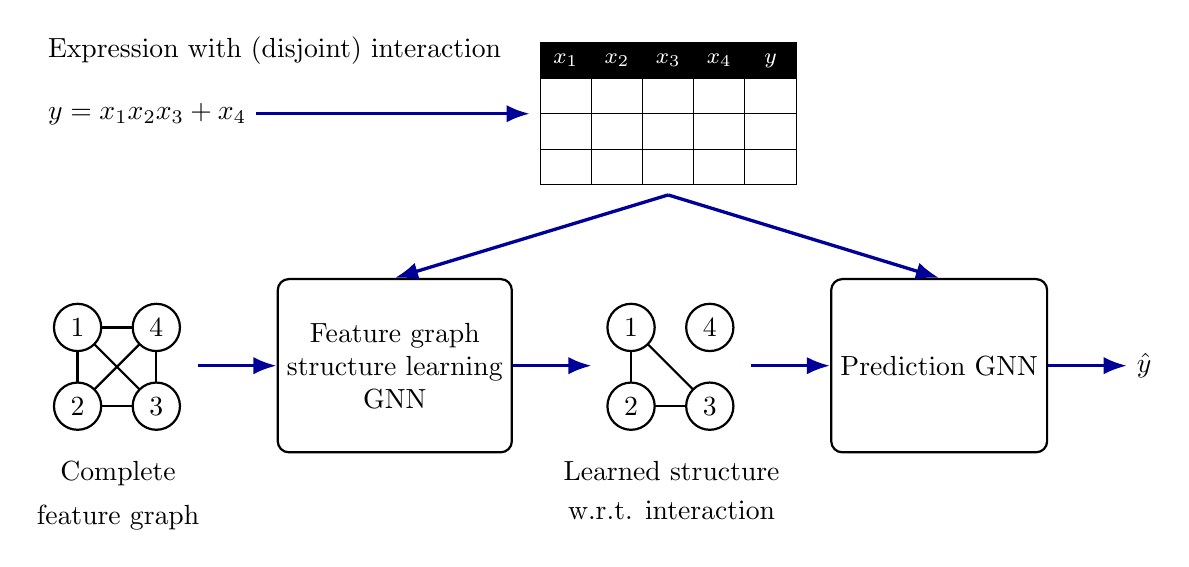
\begin{tikzpicture}[
  >=Latex,
  node distance=1.7cm and 2.0cm,
  box/.style={draw, rounded corners, minimum width=4.4cm, minimum height=2.2cm, thick, align=center},
  smallbox/.style={draw, rounded corners, minimum width=3.6cm, minimum height=2.2cm, thick, align=center},
  cap/.style={font=\footnotesize, align=center},
  arr/.style={->, very thick, blue!60!black},
  dot/.style={circle, draw, inner sep=1pt, minimum size=6mm, thick},
  every label/.style={font=\scriptsize},
]

%------------------- Top: expression and dataset -------------------
\node (exprlbl) [anchor=west] at (-6.2, 4.0) {Expression with (disjoint) interaction};
\node (expr) [anchor=west] at (-6.2, 3.2) {$y = x_1 x_2 x_3 + x_4$};

% dataset as a small matrix
\matrix (data) [matrix of nodes,
  nodes in empty cells,
  nodes={draw, minimum width=0.65cm, minimum height=0.45cm, anchor=center},
  column sep=-\pgflinewidth, row sep=-\pgflinewidth,
  row 1/.style={nodes={fill=black, text=white,font=\footnotesize\bfseries}},
  font=\scriptsize,
] at (1.8,3.2)
{
 $x_1$ & $x_2$ & $x_3$ & $x_4$ & $y$ \\
       &       &       &       &     \\
       &       &       &       &     \\
       &       &       &       &     \\
};

%------------------- Bottom row: blocks and graphs -------------------
% complete feature graph (left)
\node (complete) [smallbox, anchor=west,minimum width=2cm,minimum height=2cm, draw=none] at (-6.2,0) {};
\node (below_complete) [below=2pt of complete.south] {Complete};
\node [below=0pt of below_complete.south] {feature graph};

% nodes inside complete graph
\coordinate (c1) at ([xshift=5mm,yshift=15mm]complete.south west);
\coordinate (c2) at ([xshift=5mm,yshift=5mm]complete.south west);
\coordinate (c3) at ([xshift=15mm,yshift=5mm]complete.south west);
\coordinate (c4) at ([xshift=15mm,yshift=15mm]complete.south west);

% all pair edges (bidirected)
\draw[-, thick] (c1) -- (c2);
\draw[-, thick] (c1) -- (c3);
\draw[-, thick] (c1) -- (c4);
\draw[-, thick] (c2) -- (c3);
\draw[-, thick] (c2) -- (c4);
\draw[-, thick] (c3) -- (c4);
\node[dot,fill=white] at (c1) {1};
\node[dot,fill=white] at (c2) {2};
\node[dot,fill=white] at (c3) {3};
\node[dot,fill=white] at (c4) {4};

% structure learning block (center)
\node (learn) [smallbox, right=1cm of complete, minimum width=1cm] {Feature graph\\structure learning\\GNN};

% learned structure (right of learn)
\node (learned) [smallbox, right=1cm of learn, minimum height=2cm, minimum width = 2cm,draw=none] {};
\node (below_learned) [below=2pt of learned.south] {Learned structure};
\node[below=0.5pt of below_learned.south] {w.r.t. interaction};
% nodes inside learned graph (triangle over 1--2--3, node 4 isolated)
\coordinate (l1) at ([xshift=5mm,yshift=15mm]learned.south west);
\coordinate (l2) at ([xshift=5mm,yshift=5mm]learned.south west);
\coordinate (l3) at ([xshift=15mm,yshift=5mm]learned.south west);
\coordinate (l4) at ([xshift=15mm,yshift=15mm]learned.south west);
\draw[-, thick] (l1) -- (l2);
\draw[-, thick] (l2) -- (l3);
\draw[-, thick] (l1) -- (l3);
\node[dot,fill=white] at (l1) {1};
\node[dot,fill=white] at (l2) {2};
\node[dot,fill=white] at (l3) {3};
\node[dot,fill=white] at (l4) {4};


% prediction block (far right)
\node (pred) [smallbox, right=1cm of learned, minimum width=1cm] {Prediction GNN};
\node (yhat) [anchor=west] at ([xshift=1cm]pred.east) {$\hat{y}$};

%------------------- Arrows -------------------
\draw[arr] (expr) -- (data.west|-expr);              % expression -> dataset
\draw[arr] (data.south) -- (pred.north);                   % dataset -> prediction
\draw[arr] (data.south) -- (learn.north);                  % dataset -> learning block
\draw[arr] (complete.east) -- (learn.west);          % complete graph -> learning
\draw[arr] (learn.east) -- (learned.west);           % learning -> learned graph
\draw[arr] (learned.east) -- (pred.west);            % learned graph -> prediction
\draw[arr] (pred.east) -- (yhat.west);            % learned graph -> prediction


\end{tikzpicture}
\caption{Pipeline for attention-guided feature-graph selection and prediction. 
A complete feature graph and the training table are fed to a structure-learning GNN that outputs a sparse interaction graph (here highlighting the group $\{1,2,3\}$). 
The learned graph is then used by a prediction GNN together with the original features to produce $\hat{y}$.}
\label{fig:pipeline}
\end{figure}


We propose a minimal score--prune--retrain pipeline that selects a sparse feature--interaction graph from a complete graph using attention signals from an attention-based GNN. The design keeps assumptions and hyperparameters simple to isolate the effect of edge selection on interaction capturing. The summary of our method is described in Algorithm \ref{high-level-algor} in the Appendix.

\paragraph{Feature Graph and Model:}
Given a tabular matrix $X\in\mathbb{R}^{m\times d}$, we build a complete \emph{bi-directed} feature graph with nodes $V=\{1,\dots,d\}$ and edge set $E_{\mathrm{all}}=\{(i,j): i\neq j\}$. Interactions are evaluated on \emph{undirected} pairs $\{i,j\}$. We train a one-layer TransformerConv GNN on $E_{\mathrm{all}}$ exposes all pairwise channels so that attention can score potential interactions.

\paragraph{Attention-Derived Edge Metric:}
Let $\alpha^{(h)}_{ij}(x)$ denote the attention coefficient from feature $i$ to $j$ for head $h$ on sample $x$. We aggregate across the training set $\mathcal{S}$ and heads $h=1,\dots,H$ to obtain a directed score,
\[
\overline{A}_{ij} \;=\; \frac{1}{|\mathcal{S}|\,H} \sum_{x\in\mathcal{S}} \sum_{h=1}^H \alpha^{(h)}_{ij}(x),
\]
then symmetrize to reflect undirected interactions,
\[
M_{ij} \;=\; \tfrac{1}{2}\big(\overline{A}_{ij} + \overline{A}_{ji}\big), \quad i\neq j.
\]
Finally, we apply a min--max normalization over unordered pairs to obtain the interaction metric used for selection,
\[
M^{\mathrm{F}}_{ij} \;=\; \mathrm{MinMaxNorm}\!\big( M_{ij} : 1 \le i < j \le d \big),
\]
which we abbreviate as the “MF” score. Larger $M^{\mathrm{F}}_{ij}$ indicates stronger evidence that features $i$ and $j$ participate in the same interaction group.

\paragraph{Edge Selection via Global Threshold:}
We select a sparse undirected edge set by thresholding the MF score,
\[
E_\tau \;=\; \big\{ \{i,j\} : M^{\mathrm{F}}_{ij} \ge \tau \big\}.
\]
On the synthetic dataset with ground-truth edges $E^\star$, the threshold $\tau$ is chosen on the validation split to maximize edge-level $F_1(E_\tau, E^\star)$ (or to match a sparsity budget when required). Ties are broken by keeping the larger $M^{\mathrm{F}}_{ij}$. For training the predictor on the pruned graph, we convert $E_\tau$ to a symmetric directed edge set.

\paragraph{Retraining on the Pruned Graph:}
After selection, we retrain the same architecture \emph{from scratch} on the pruned edge set with the same optimizer and early stopping. This avoids potential bias from continuing to train on the dense graph and yields a cleaner comparison between complete and pruned graphs.

\section{Experimental Setup}
Our experiments are designed to answer three questions: (i) do attention scores expose the true interaction structure on the synthetic dataset; (ii) can a simple global threshold recover most ground-truth edges while keeping the graph sparse; and (iii) does pruning preserve predictive performance relative to a complete graph under identical training settings.

\paragraph{Dataset and Splits:}
We use the complex case introduced by prior work. The target is generated by
\begin{equation}
\label{eq:complex}
\small
 y := \frac{1}{1 + x_0^2 + x_1^2 + x_2^2} + \sqrt{\exp(x_3 + x_4)} + |x_5 + x_6| + x_7 x_8 x_9 .
\end{equation}
We then draw $m=10{,}000$ i.i.d.\ samples by sampling each feature $x_j \sim \mathcal{U}[-1,1]$ independently ($j=0,\ldots,9$) and computing $y$ from Eq.~\eqref{eq:complex}.
The ground-truth interaction groups are $\{x_0,x_1,x_2\}$, $\{x_3,x_4\}$, $\{x_5,x_6\}$, and $\{x_7,x_8,x_9\}$. We evaluate recovery of these groups using pairwise edges and simple metrics. Expected feature graph is as follow:
\begin{center}
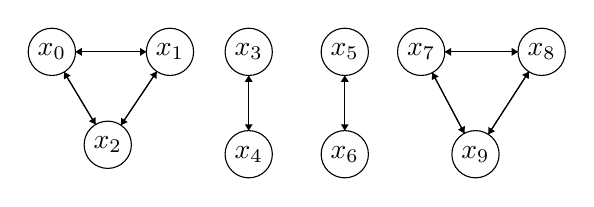
\begin{tikzpicture}[scale=0.1]
\tikzstyle{every node}+=[inner sep=0pt]
\draw [black] (14.9,-13.6) circle (3);
\draw (14.9,-13.6) node {$x_0$};
\draw [black] (29.9,-13.6) circle (3);
\draw (29.9,-13.6) node {$x_1$};
\draw [black] (22,-25.4) circle (3);
\draw (22,-25.4) node {$x_2$};
\draw [black] (39.9,-13.6) circle (3);
\draw (39.9,-13.6) node {$x_3$};
\draw [black] (39.9,-26.6) circle (3);
\draw (39.9,-26.6) node {$x_4$};
\draw [black] (52.1,-13.6) circle (3);
\draw (52.1,-13.6) node {$x_5$};
\draw [black] (52.1,-26.6) circle (3);
\draw (52.1,-26.6) node {$x_6$};
\draw [black] (61.8,-13.6) circle (3);
\draw (61.8,-13.6) node {$x_7$};
\draw [black] (77.1,-13.6) circle (3);
\draw (77.1,-13.6) node {$x_8$};
\draw [black] (68.7,-26.6) circle (3);
\draw (68.7,-26.6) node {$x_9$};
\draw [black] (16.45,-16.17) -- (20.45,-22.83);
\fill [black] (20.45,-22.83) -- (20.47,-21.89) -- (19.61,-22.4);
\draw [black] (20.45,-22.83) -- (16.45,-16.17);
\fill [black] (16.45,-16.17) -- (16.43,-17.11) -- (17.29,-16.6);
\draw [black] (17.9,-13.6) -- (26.9,-13.6);
\fill [black] (26.9,-13.6) -- (26.1,-13.1) -- (26.1,-14.1);
\draw [black] (26.9,-13.6) -- (17.9,-13.6);
\fill [black] (17.9,-13.6) -- (18.7,-14.1) -- (18.7,-13.1);
\draw [black] (23.67,-22.91) -- (28.23,-16.09);
\fill [black] (28.23,-16.09) -- (27.37,-16.48) -- (28.2,-17.04);
\draw [black] (28.23,-16.09) -- (23.67,-22.91);
\fill [black] (23.67,-22.91) -- (24.53,-22.52) -- (23.7,-21.96);
\draw [black] (39.9,-23.6) -- (39.9,-16.6);
\fill [black] (39.9,-16.6) -- (39.4,-17.4) -- (40.4,-17.4);
\draw [black] (39.9,-16.6) -- (39.9,-23.6);
\fill [black] (39.9,-23.6) -- (40.4,-22.8) -- (39.4,-22.8);
\draw [black] (52.1,-16.6) -- (52.1,-23.6);
\fill [black] (52.1,-23.6) -- (52.6,-22.8) -- (51.6,-22.8);
\draw [black] (52.1,-23.6) -- (52.1,-16.6);
\fill [black] (52.1,-16.6) -- (51.6,-17.4) -- (52.6,-17.4);
\draw [black] (67.29,-23.95) -- (63.21,-16.25);
\fill [black] (63.21,-16.25) -- (63.14,-17.19) -- (64.02,-16.72);
\draw [black] (63.21,-16.25) -- (67.29,-23.95);
\fill [black] (67.29,-23.95) -- (67.36,-23.01) -- (66.48,-23.48);
\draw [black] (70.33,-24.08) -- (75.47,-16.12);
\fill [black] (75.47,-16.12) -- (74.62,-16.52) -- (75.46,-17.06);
\draw [black] (75.47,-16.12) -- (70.33,-24.08);
\fill [black] (70.33,-24.08) -- (71.18,-23.68) -- (70.34,-23.14);
\draw [black] (64.8,-13.6) -- (74.1,-13.6);
\fill [black] (74.1,-13.6) -- (73.3,-13.1) -- (73.3,-14.1);
\draw [black] (74.1,-13.6) -- (64.8,-13.6);
\fill [black] (64.8,-13.6) -- (65.6,-14.1) -- (65.6,-13.1);
\end{tikzpicture}
\end{center}
We use the complex synthetic case defined in Eq.~\eqref{eq:complex}, which specifies four higher-order interaction groups. Inputs are generated independently and standardized before training. We run on first 80\% train and last 20\% test.


\paragraph{Feature-Graph Dataset Construction:}
Given $d$ features and an edge set $E$, we build a graph dataset for training by pairing each tabular sample with the feature graph. Let $x$ denote the per-sample feature vector and $X$ a learnable per-node embedding matrix. The initial node representation is
\begin{equation}
H^{(0)} \;=\; \mathrm{concat}(x, X).
\end{equation}
For the main results, we use raw feature values (optionally standardized) concatenated with $X$.


\paragraph{Baselines:}
We compare against: (1) \textbf{GNN (Complete)} trained on the fully connected feature graph; (2) \textbf{Oracle (Ground Truth)} using the known edge set $E^\star$; and (3) \textbf{Null Graph} and (4) \textbf{Ablation one expected edge}. These baselines isolate the effect of edge selection.


\paragraph{Metrics:}
\textbf{Interaction recovery.} Let $\widehat{E}$ be the selected edge set and $E^\star$ the ground truth. We compute \emph{Precision}$=\tfrac{|\widehat{E} \cap E^\star|}{|\widehat{E}|}$, \emph{Recall}$=\tfrac{|\widehat{E} \cap E^\star|}{|E^\star|}$, and $F_1=\tfrac{2\cdot \mathrm{Precision}\cdot \mathrm{Recall}}{\mathrm{Precision}+\mathrm{Recall}}$. \textbf{Prediction.} We report average MAE on the held-out test set from 10 times of experiment for each graph setting.


\paragraph{Training Protocol:}
All models share the same architecture and training settings: one-layer TransformerConv (hidden 128), ReLU, Adam (adpative with initial lr $10^{-3}$), batch size 128, up to 2000 epochs with early stopping on validation loss. For threshold selection, we sweep a small set of candidates $\mathcal{T}$ and choose $\tau$ on validation to maximize $F_1(E_\tau, E^\star)$ (or to meet a sparsity target when specified). After selection, the predictor is retrained from scratch on the pruned graph.

\section{Results}

Figure \ref{fig:result1} shows the $M_{ij}$ heatmap, which clearly highlights the four interaction groups in \Cref{eq:complex}.
With a threshold $\tau{=}0.68$, we obtain
\[
E_\tau = \{\{0,1\}, \{0,2\}, \{1,3\}, \{1,9\}, \{3,4\}, \{5,6\}, \{7,8\}, \{7,9\}, \{8,9\}\},
\]
which almost matches the ground truth; $\{1,9\}$ is spurious. The number of edges is small compared to the complete graph (only 20\% density compared to the complete graph). We get 0.89 precision, 1.00 recall and 0.94 F1-score at this threshold.

\paragraph{Prediction Performance}
We compare predictors trained on different feature graphs while keeping the architecture and training settings identical. The variants are: (i) \textbf{Complete} — a fully connected feature graph; (ii) \textbf{Ground Truth (Oracle)} — the known interaction edge set $E^\star$; (iii) \textbf{Null} — no edges (message passing disabled); and (iv) \textbf{Pruned (Global Threshold)} — the selected edges $E_\tau$ from our method (here $\tau{=}0.68$). We report regression error on the synthetic task.

Models trained on the pruned graph match or improve upon the complete graph and approach the oracle, while the null graph performs significantly worse. This supports the hypothesis that removing noisy edges improves generalization without harming predictive accuracy \cite{Yamchote2025FromFT}.

\begin{paracol}{2}
% LEFT column
\begin{leftcolumn}
\centering
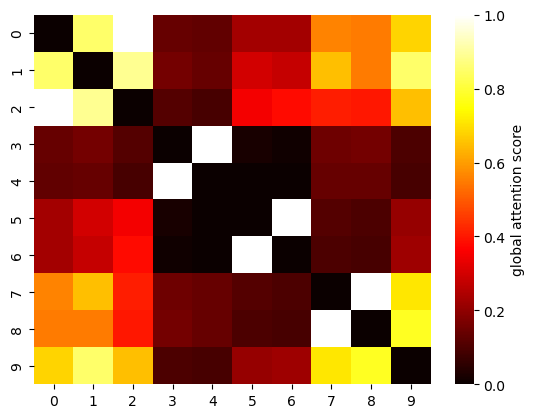
\includegraphics[width=\linewidth]{result1-3-new.png}
\captionof{figure}{$M^{\mathrm{F}}$ (0–1, averaged over heads/samples). 
Bright blocks at \{0,1,2\}, \{3,4\}, \{5,6\}, \{7,8,9\} recover the ground-truth groups; diagonal shown but not evaluated.}
\label{fig:result1}
\end{leftcolumn}

% RIGHT column
\begin{rightcolumn}
\centering
\footnotesize

\label{tab:synthetic-prediction}
\begin{tabular}{lc}
  \toprule
  \textbf{Graph Type} & \textbf{MAE} \\
  \midrule
  Pruned ($\tau{=}0.68$) & 0.072 \\
  \midrule
  Ground Truth (Oracle) & 0.070 \\
  Complete              & 0.088 \\
  Null (no edges)       & 0.397 \\
  \midrule
  $[3,4],[5,6],[7,8,9]$   & 0.079 \\
  $[0,1,2],[3,4],[7,8,9]$ & 0.091 \\
  $[0,1,2],[5,6],[7,8,9]$ & 0.097 \\
  $[5,6],[7,8,9]$       & 0.101 \\
  $[0,1,2],[7,8,9]$     & 0.117 \\
  $[0,1,2],[3,4],[5,6]$ & 0.155 \\
  $[0,1,2],[3,4]$       & 0.162 \\
  $[3,4],[5,6]$         & 0.166 \\
  $[0,1,2],[5,6]$       & 0.173 \\
  $[5,6]$               & 0.176 \\
  $[3,4],[7,8,9]$       & 0.356 \\
  $[7,8,9]$             & 0.365 \\
  $[3,4]$               & 0.389 \\
  $[0,1,2]$             & 0.398 \\
  \bottomrule
\end{tabular}
\captionof{table}{Prediction performance (MAE in average of 10 runnings) on the synthetic regression dataset sorted by MAE score from lowest to highest of each view.}
\end{rightcolumn}
\end{paracol}


\section{Discussion}
This study asks whether an attention-based GNN can (i) capture interaction groups and (ii) select a sparse feature graph without interrupting prediction on a dataset with known ground truth. On the complex synthetic case, the answer is positive: a single global threshold on an attention-derived score (MF) recovers most true edges (Precision $0.89$, Recall $1.00$, $F_1=0.94$) and yields a compact graph (9 vs.\ 45 edges) with competitive MAE ($0.072$ vs.\ $0.088$ for the complete graph, $0.070$ oracle).

\paragraph{Why selection helps.}
Training on a complete graph exposes every pairwise channel, but also introduces many weak or noise edges. Pruning removes these noisy signal, reducing variance in message passing and simplifying the hypothesis space. The result is a small accuracy gain (MAE $0.072$ vs.\ $0.088$) together with a large reduction in edge count.

\paragraph{Structure discovery and pairwise proxies.}
The attention heatmap shows clear blocks matching the four interaction groups, and the selected edges connect almost all members inside each group. Although the ground truth includes higher-order terms, pairwise edges were sufficient proxies in this dataset: dense within-group connectivity emerged without requiring explicit $k$-way operators.

\paragraph{Error analysis.}
One spurious edge (\{1,9\}) appears in the recovered set. This can occur when features co-vary under the generative process or when attention aggregates across shared downstream effects during training. Such edges are rare here (Precision $0.89$), but they highlight the model dependence of attention scores.

\paragraph{Ablation insights.}
The prediction table with partial group combinations indicates that interactions involving $\{3,4\}$ and $\{7,8,9\}$ contribute most to accuracy (e.g., $\{3,4\},\{5,6\},\{7,8,9\}$ reaches MAE $\approx 0.079$), while the $\{0,1,2\}$ term shows lower marginal utility on its own or when paired with fewer groups. This aligns with the functional form where some terms have stronger effect sizes.

\paragraph{Future work.}
Promising directions include stability selection without ground truth in the real-world case, combining attention with structural priors or regularizers, explicit higher-order (hyperedge) scoring, and scaling studies for larger $d$ and noisier regimes.

\section{Conclusion}
The study investigates whether an attention-based GNN can identify interaction groups and select a sparse feature graph without compromising prediction accuracy on a dataset with known ground truth. Results show that using a global threshold on an attention-derived score can successfully recover most true edges, creating a compact graph with significantly fewer edges while maintaining competitive Mean Absolute Error (MAE). Training on a complete graph introduces unnecessary noisy edges, but pruning these edges reduces variance and helps in hypothesis simplification, thus slightly improving accuracy. The attention heatmap visually correlates with interaction groups, establishing that dense within-group connectivity could be captured with pairwise edges, despite the presence of higher-order terms in ground truth. The emergence of a spurious edge exemplifies the model's attention score dependency, although such edges are infrequent. The threshold setting balances between precision and recall, maintaining prediction quality with multiple sparse graphs around this threshold. Integrating attention scores with domain knowledge highlights particular interactions contributing significantly to predictive accuracy. Reducing the edge count improves memory efficiency and interpretability of interactions. Future directions include developing methods for stability selection without ground truth, integrating attention with structural priors or regularizers, exploring hyperedge scoring, and scaling GNNs to broader applications and noisier conditions.

% End

\bibliographystyle{IEEEtran}
\bibliography{sample701.bib}


\newpage
\appendix
\section{Appendix}
\subsection{Algorithm of our Method}
\begin{algorithm}[h!]
\caption{Attention-Guided Feature–Interaction Graph Selection}\label{high-level-algor}
\begin{algorithmic}[1]
\Require $(X,y)$ with $X\in\mathbb{R}^{m\times d}$, $y\in\mathbb{R}^m$; complete directed edge set $E_{\mathrm{all}}=\{(i,j):\, i\neq j,\ i,j\in[d]\}$; candidate thresholds $\mathcal{T}\subset[0,1]$; (synthetic only) ground-truth undirected edge set $E^\star$
\Ensure Sparse undirected edge set $E_{\tau^\star}$ and predictor $f_{\hat\theta_{\tau^\star}}$
\State \textbf{Fit on complete graph:} 
\[
\hat\theta_{\mathrm{all}}\in\arg\min_{\theta}\ \frac{1}{m}\sum_{t=1}^{m}\ell\!\big(f_\theta(x^{(t)};\,E_{\mathrm{all}}),\,y^{(t)}\big).
\]
\vspace{-0.3em}
\State \textbf{Attention aggregation:} For each unordered pair $\{i,j\}$ with $1\le i<j\le d$, let $\alpha^{(h)}_{ij}(x;\hat\theta_{\mathrm{all}})$ be the attention from $i\!\to\! j$ for head $h\in[H]$ on sample $x$. Define
\[
\overline{A}_{ij}\;=\;\frac{1}{|\mathcal{S}_{\mathrm{train}}|\,H}\sum_{x\in\mathcal{S}_{\mathrm{train}}}\ \sum_{h=1}^{H}\alpha^{(h)}_{ij}(x;\hat\theta_{\mathrm{all}}),\qquad
M_{ij}\;=\;\tfrac{1}{2}\big(\overline{A}_{ij}+\overline{A}_{ji}\big).
\]
\vspace{-0.3em}
\State \textbf{Normalization (MF score):} Over all $1\le p<q\le d$, set
\[
M^{\mathrm{F}}_{ij}\;=\;\frac{M_{ij}-\min_{p<q}M_{pq}}{\max_{p<q}M_{pq}-\min_{p<q}M_{pq}},\qquad (1\le i<j\le d).
\]
\vspace{-0.3em}
\State \textbf{Thresholded graphs:} For each $\tau\in\mathcal{T}$, define the undirected edge set
\[
E_{\tau}\;=\;\big\{\{i,j\}\ :\ M^{\mathrm{F}}_{ij}\ge\tau,\ 1\le i<j\le d\big\}.
\]
\vspace{-0.3em}
\State \textbf{Model selection (validation):} 
\[
\tau^\star\in\arg\max_{\tau\in\mathcal{T}}\ F_1\!\big(E_{\tau},\,E^\star\big)
\quad\text{(or }\ \arg\max_{\tau\in\mathcal{T}}F_1\ \text{s.t. }|E_{\tau}|\le B\text{ for a budget }B\text{)}.
\]
\vspace{-0.3em}
\State \textbf{Symmetric directed edge set for training:}\ 
$$\vec{E}_{\tau^\star}=\{(i,j):\{i,j\}\in E_{\tau^\star}\}\cup\{(j,i):\{i,j\}\in E_{\tau^\star}\}$$.
\vspace{-0.3em}
\State \textbf{Retrain on pruned graph:}
\[
\hat\theta_{\tau^\star}\in\arg\min_{\theta}\ \frac{1}{m}\sum_{t=1}^{m}\ell\!\big(f_\theta(x^{(t)};\,\vec{E}_{\tau^\star}),\,y^{(t)}\big).
\]
\vspace{-0.3em}
\State \textbf{return} $E_{\tau^\star}$ and $f_{\hat\theta_{\tau^\star}}$.
\end{algorithmic}
\end{algorithm}

\subsection{Used GNN Model}
Our GNN model utilizes transformer convolution layers (TransformerConv \cite{TransformerConv}) for the message passing function, incorporating attention mechanisms to capture the strength of pairwise interactions. Then, a mean pooling layer averages the embedding of all nodes for the prediction layer.

As Fi-GNN does, this work adopts the idea from Fi-GNN, but with a simpler architecture. We use TransformerConv \cite{TransformerConv}, which is a message-passing layer based on the attention mechanism, whose feature interaction learning capability is shown by many works. For the computation, we start from the initial node embedding $H^{(0)}$. Then, a feature graph with the node embedding matrix is fed to TransformerConv with BatchNorm:
\begin{equation} \label{eq:transformerConv}
\begin{split}
    Z^{(l)} &= \text{TransformerConv}(H^{(l-1)},E),\\
    H^{(l)} &= \text{ReLU}(\text{BatchNorm}(Z^{(l)})),
\end{split}
\end{equation}
where $H^{(l)}$ is an intermediate node embedding matrix at the layer $l$. After applying all message passing layers, we calculate the average pooling of node embeddings from the last GNN layer, and we use this vector as a graph embedding, which is fed into the projection layer to get a prediction:
\begin{align} 
    \vec{p} &= \frac{1}{n}\sum_{i}H^{(L)}[i],\label{eq:pooling}\\
    \hat{y}  &= \vec{w}\cdot \vec{p} + b,\label{eq:finalProjection}
\end{align}
where $H^{(L)}$ is a node embedding matrix from the last GNN layer and $H^{(L)}[i]$ is the row $i$ of the matrix which corresponds to the node embedding of the node $i$ and $b$ is a biased term. Equation \ref{eq:pooling} is the calculation of the mean pooling layer, and Equation \ref{eq:finalProjection} is the final projection to calculate the prediction value.

\subsection{Result on Pairwise Interaction}
With the same setting of the experiment, but simpler interaction complexity datasets, we get the same result as shown in our Results section.
Below illustrates the result on datasets containing only pairwise interaction (Left) $x_0x_1 + \cdots + x_{12}x_{13} + x_{14} + \cdots + x_{23}$ and (Right) $x_0x_1 + \cdots + x_{8}x_{9} + x_{10} + \cdots + x_{24}$. Our method is extremely effective in capturing the pairwise mode of interactions.

\begin{figure}[h!]
    \centering
    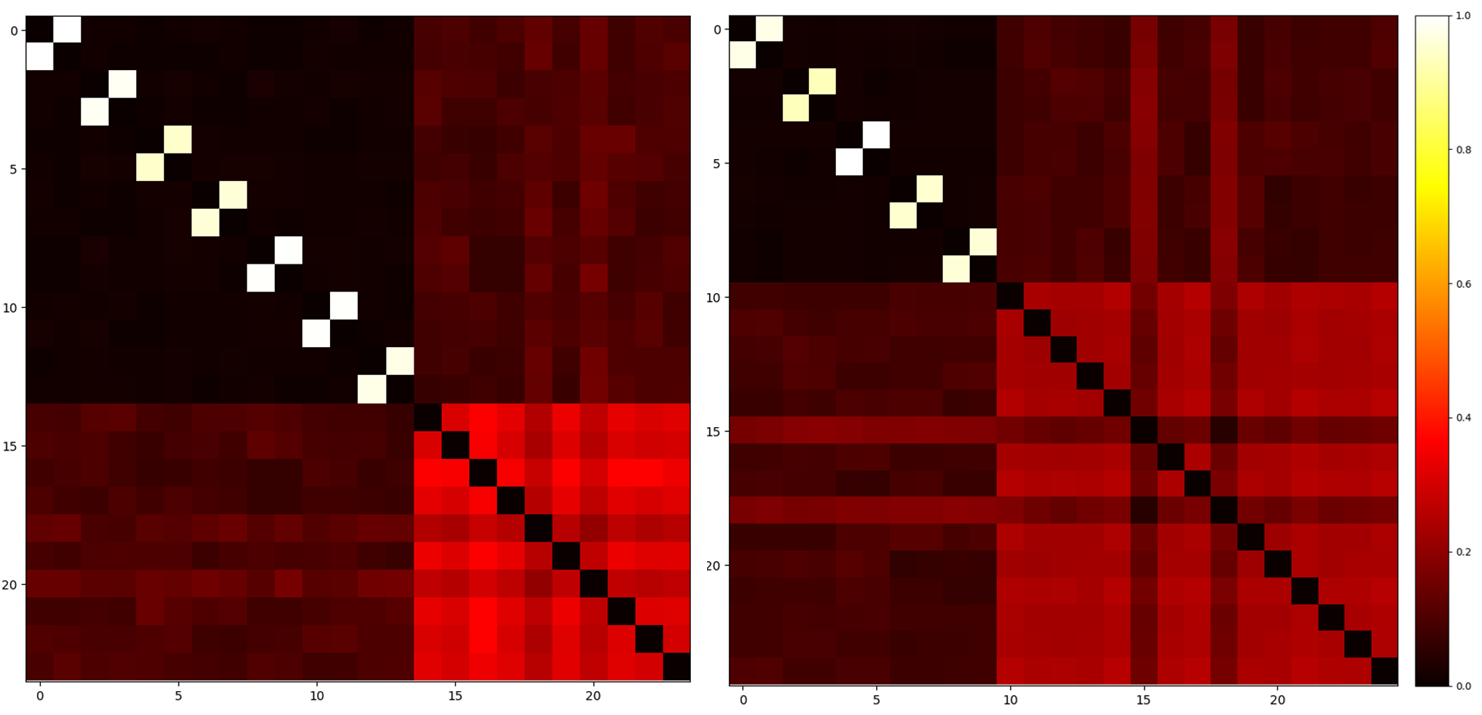
\includegraphics[width=0.8\linewidth]{result1-total.png}
    \caption{\textbf{Pairwise-interaction datasets.} Global attention heatmaps $M^{\mathrm F}$ (0–1, averaged over heads/samples). 
    Left: disjoint pairs $(0,1),(2,3),\ldots,(12,13)$ with remaining features as main effects; 
    Right: pairs $(0,1),\ldots,(8,9)$ with the rest as main effects. 
    Bright $2\times2$ off-diagonal blocks recover the interacting pairs (diagonal shown but not evaluated).}
    \label{fig:placeholder}
\end{figure}

\end{document}
